\documentclass[english,edition=2026]{zpiday}
%\documentclass[polish,edition=2025]{zpiday}

\usepackage{lipsum}
\title{Building Irregularity Recognition and Detection}
\acronym{BIRD}
\supervisor{dr hab. inż. Marek Krótkiewicz, prof. uczelni, Faculty of Information and Communication Technology, Wrocław University of Science and Technology}
\members{Norman Wiese\and Wojciech Górczyński\and Antoni Chorążyczewski\and Kamil Jankowski}
\projectLogo{images/icon.png}


\begin{document}


\maketitle

\begin{abstract}
In the era of increasingly fast construction times, local governments and property owners struggle to keep their records accurate with reality. The rapid development of rural areas, combined with the limitations of traditional inspection methods, result in flawed records.\par
The main objective of the project is to reduce the costs and time associated with identifying these inconsistencies manually using traditional building verification methods, while improving the accuracy of official property records. By automating the initial stages of the inspection process, the platform will allow institutions to focus on cases that require further investigation.\par
This goal will be accomplished using a trained AI model that will analyze imagery obtained from orthophotomaps and identify objects of interest. The software will be delivered through a SaaS model, making it accessible through a web browser. The product is to be used by both technical and non-technical employees.\par


\end{abstract}


\section{Development}

\subsection{Introduction}
The most advanced part of the project is the development of a building footprint segmentation model. The model is trained to identify building footprints in aerial imagery, which can then be used to detect irregularities in official property records. The model is based on the SegFormer architecture and is trained using a combination of high-resolution RGB orthophotos and colour-infrared orthophotos obtained from the Polish Geoportal.\par
The remaining components of the project include a web application for visualizing the results of the model and a backend service for processing the imagery and storing the results. The web application is built using modern web technologies and is designed to be user-friendly and accessible to both technical and non-technical users.\par

\subsection{Building footprint segmentation model}
The building footprint segmentation model was developed as a dedicated
component for the analysis of aerial imagery. Its purpose is to
classify every pixel of an orthophoto as either belonging to a building or to
the background. This formulation was selected to provide a detailed
description of building geometry, which can later be converted into vector
objects and compared with existing spatial data.

\subsubsection{Training data preparation}
\par
The training data was prepared using official resources provided by the Polish
Geoportal. Downloaded orthophotos for selected areas of interest were
combined with building polygons from the BDOT10k dataset. The building
polygons were rasterised into binary masks aligned with the corresponding
orthophoto tiles. Two imagery sources were supported during dataset
construction: high-resolution RGB orthophotos obtained through the Web
Coverage Service (WCS) and colour-infrared orthophotos obtained from the
Geoportal orthophoto index.\par
The resulting data consists of image--mask pairs. The source tiles are divided
into square crops of $512 \times 512$ pixels, which corresponds to the input
size used during training. Instead of storing every crop as a separate image
file, the preparation script creates CSV manifests. Each manifest entry
contains the source image and mask paths together with the crop coordinates
and dimensions. This approach reduces storage requirements while preserving
the ability to load individual samples efficiently.\par

The samples are divided into training, validation, and test subsets using
geographic blocks. Consequently, neighbouring crops from the same geographic
area are not distributed across different subsets, reducing the risk of
overestimating model performance due to spatially correlated samples. The
sampling procedure also includes positive, mixed, and background crops so that
the model learns both building regions and difficult non-building regions.\par
\begin{figure}[h]
    \centering
    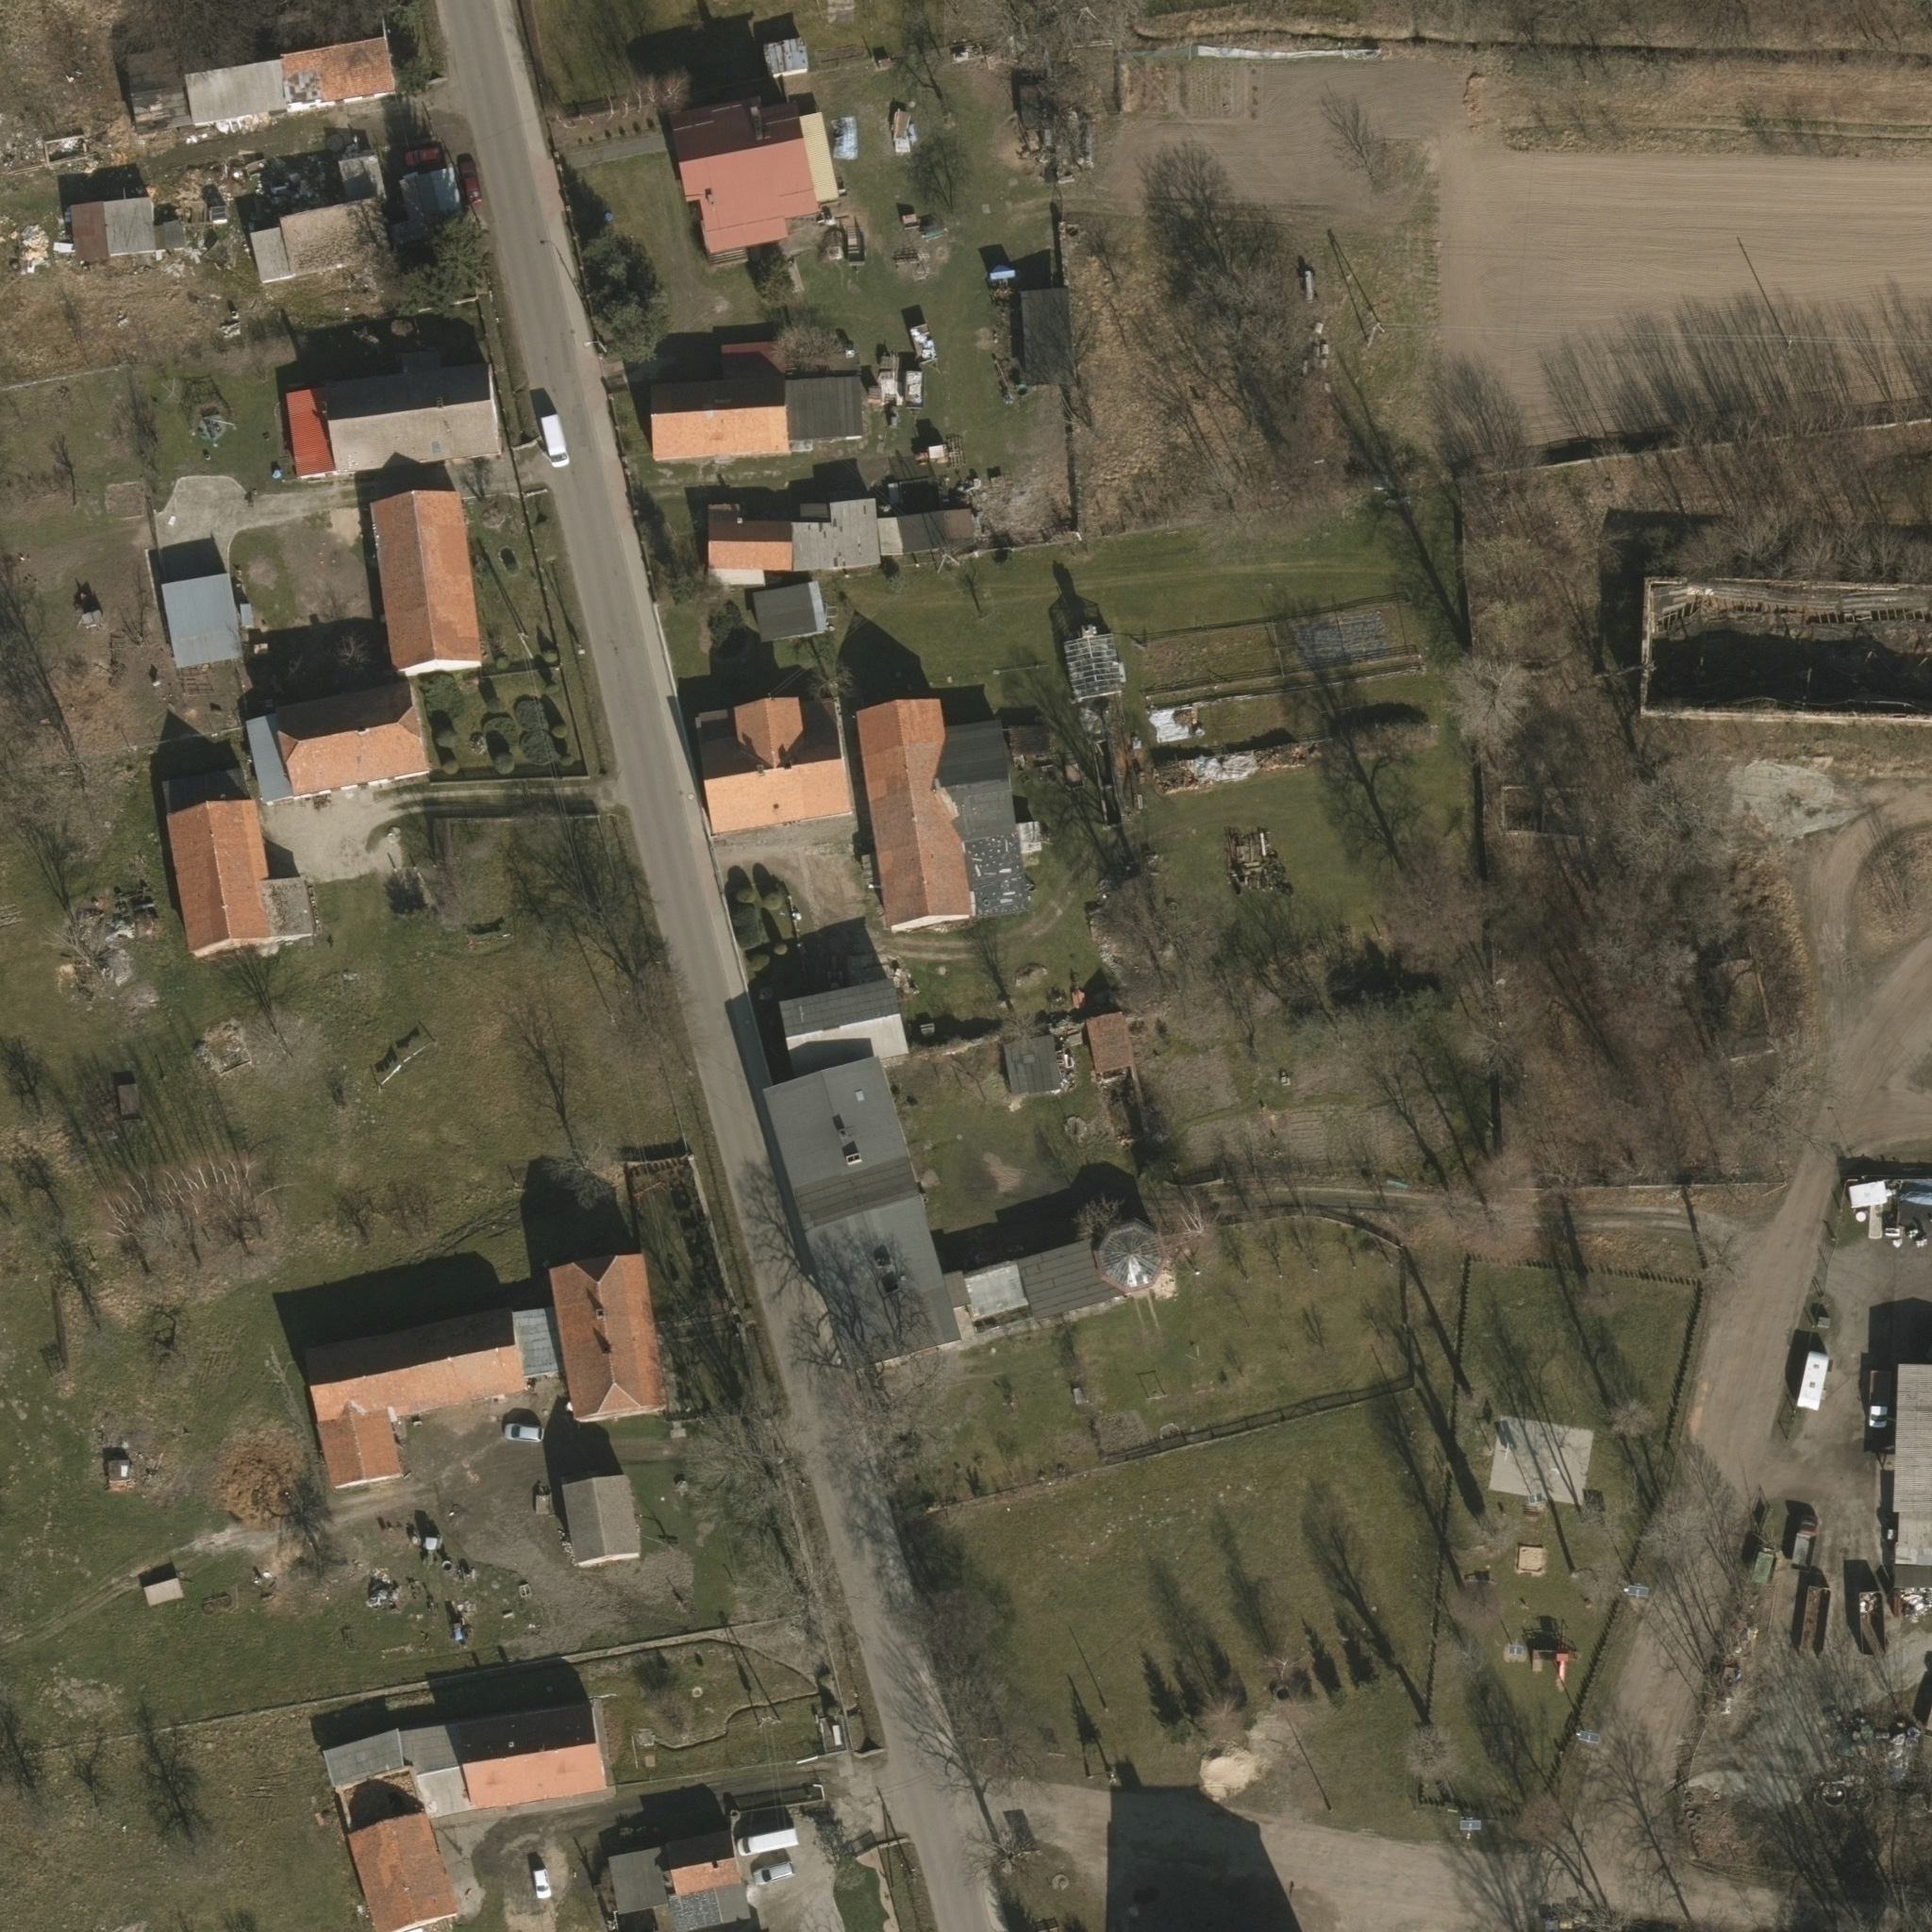
\includegraphics[width=0.45\linewidth]{images/model/tile_029_006.jpg}
    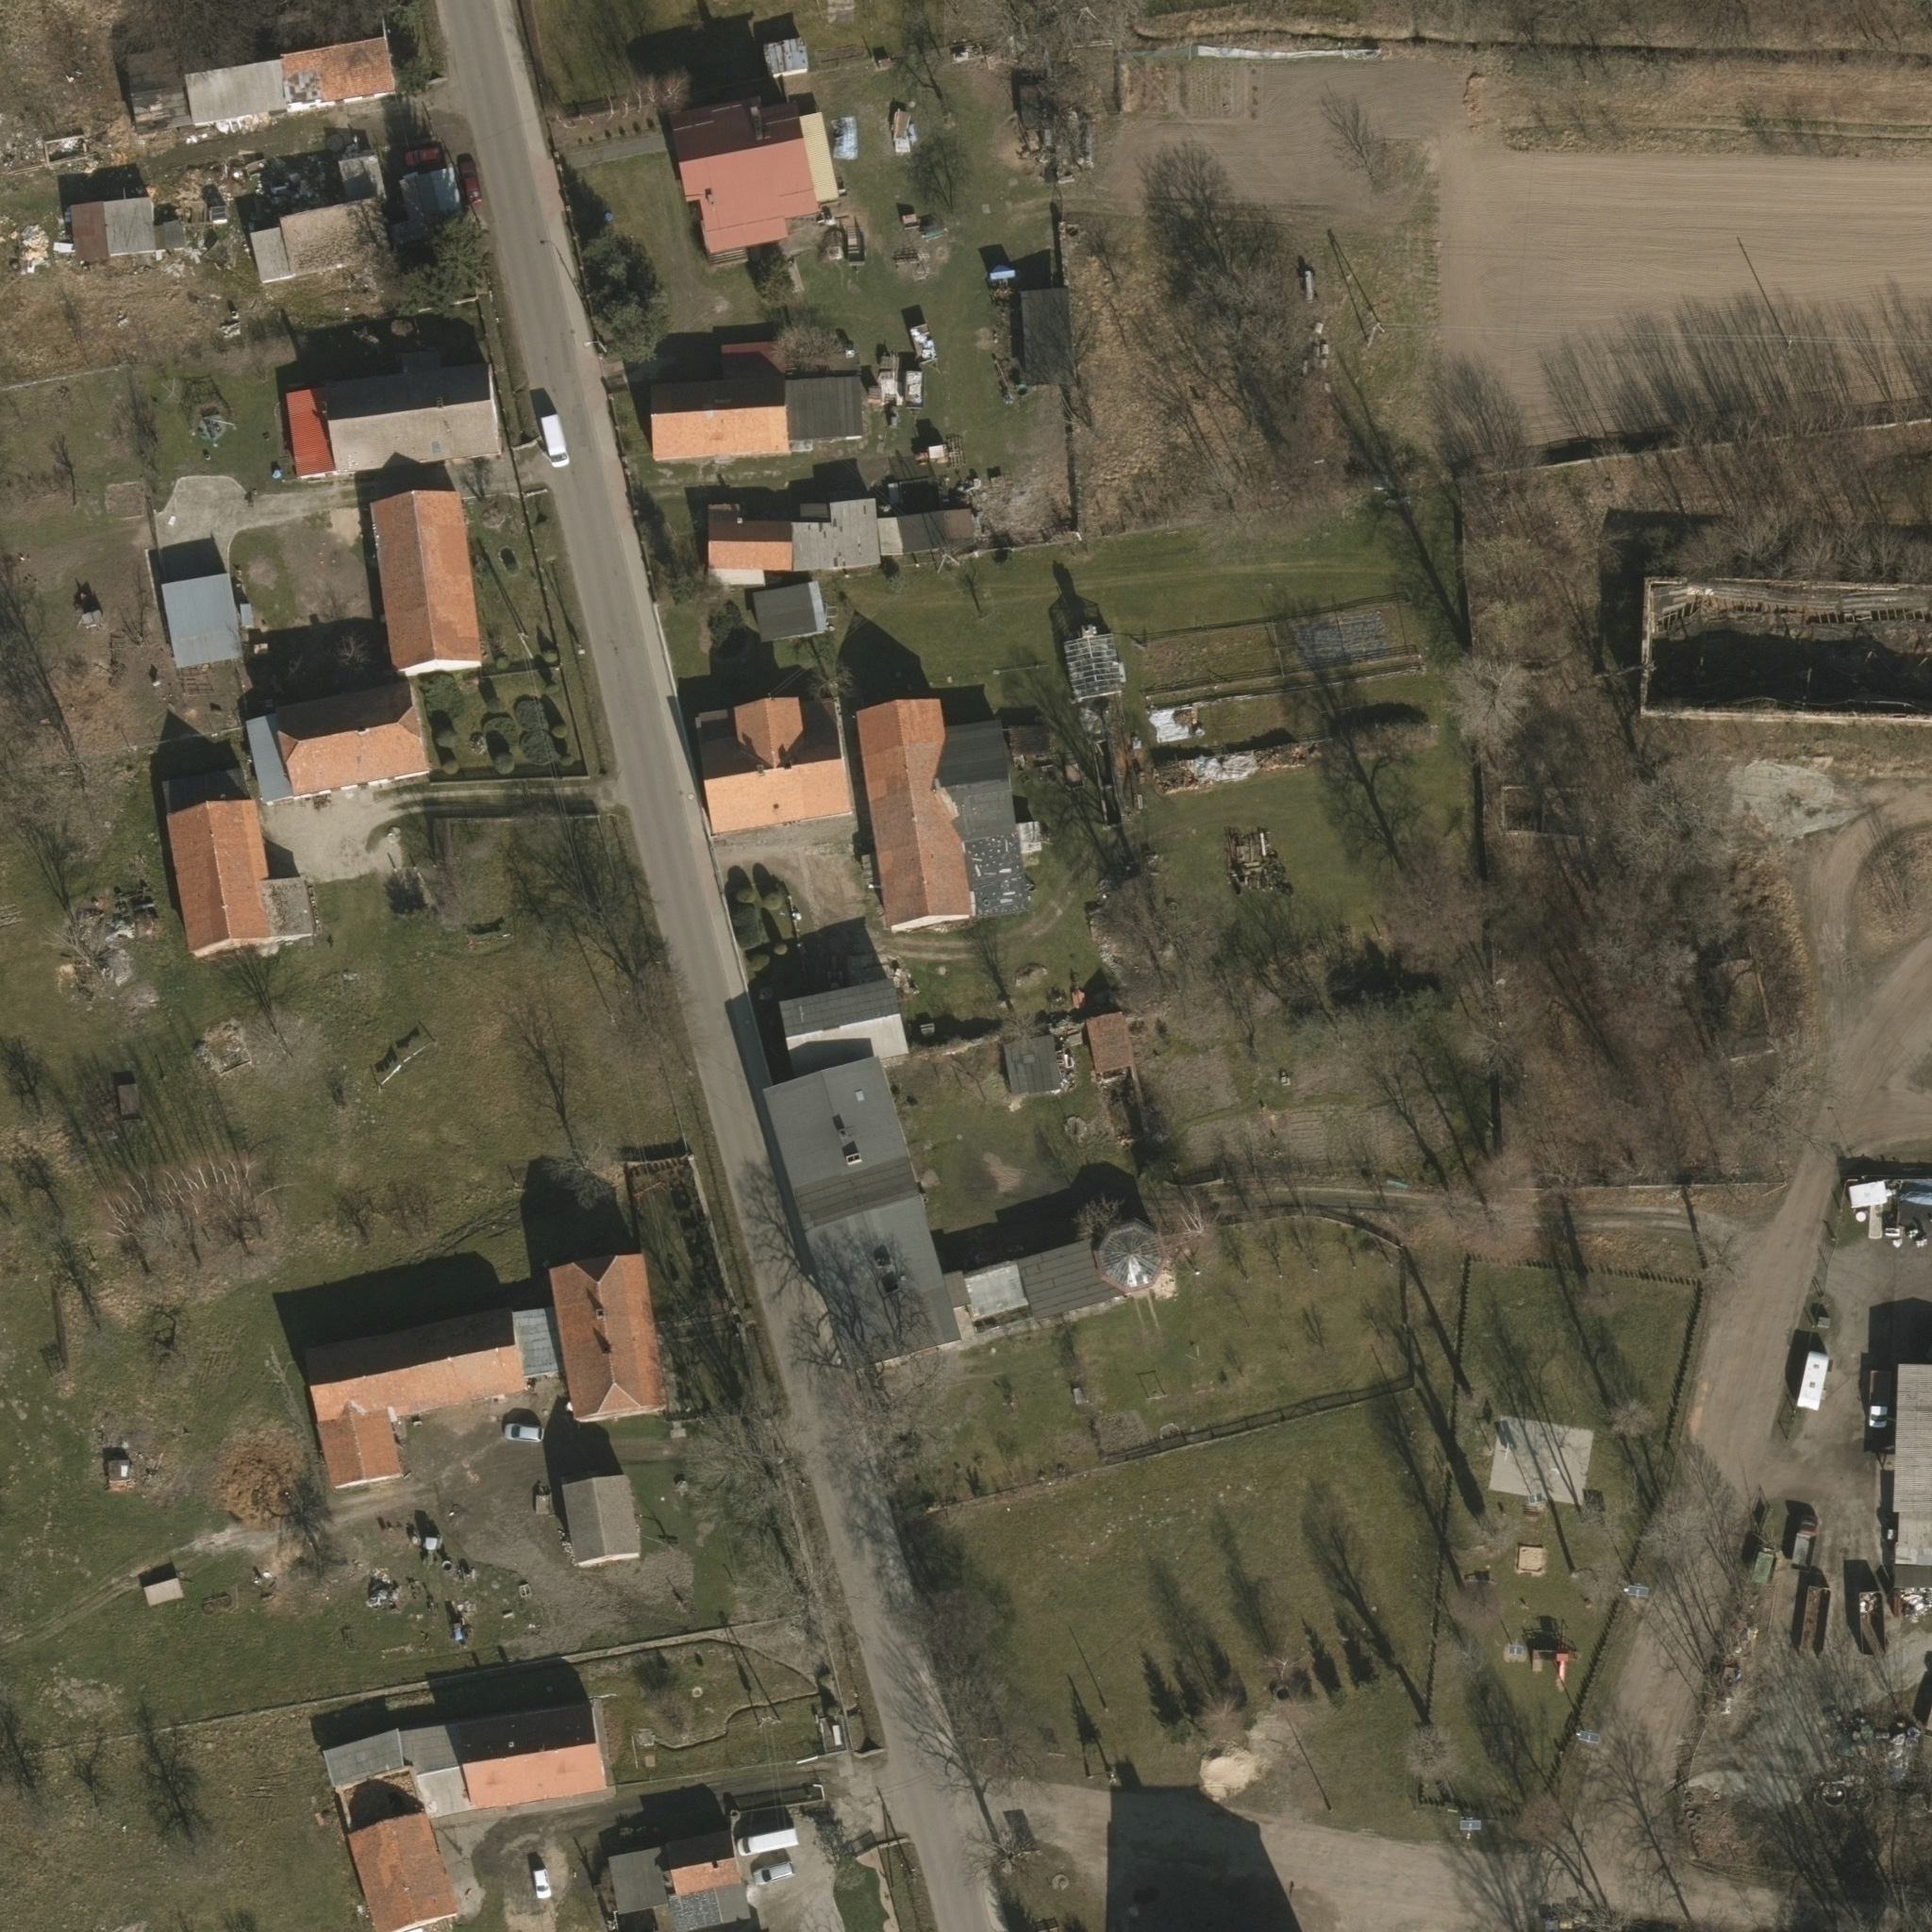
\includegraphics[width=0.45\linewidth]{images/model/tile_029_006.jpg}
    \caption{Example of training data used for building footprint segmentation. The left image is an RGB orthophoto, while the right image is a binary mask derived from the BDOT10k building polygons.}
    \label{fig:zpi-day}
\end{figure}

\subsubsection{Model architecture and training}
The model is based on the SegFormer semantic-segmentation architecture. A
pre-trained MiT encoder is used to extract features from the orthophotos and
is combined with a binary segmentation head. The default configuration uses
the NVIDIA MiT-B2 encoder; the training script allows another compatible
encoder checkpoint to be selected when required by an experiment.\par

During training, image and mask crops are loaded directly from the original
tiles according to the manifest coordinates. Data augmentation is applied to
the training subset and consists of horizontal and vertical flips, rotations
by multiples of $90^\circ$, and moderate changes to brightness, contrast,
colour saturation, and image noise. The same spatial transformation is
applied to the image and its mask, while photometric transformations are
applied only to the image. These operations increase the variability of the
training data without changing the target building geometry.\par

The optimisation objective combines binary cross-entropy with Dice loss. The
first component penalises incorrect pixel-wise classifications, while the
second improves the overlap between predicted and reference building regions.
The model is optimised with AdamW and a cosine learning-rate schedule with a
warm-up period. Gradient accumulation and mixed-precision execution are
supported to reduce GPU memory usage and enable training on consumer-grade
hardware.\par

\subsubsection{Evaluation and experiment outputs}
After every training epoch, the model is evaluated on the validation subset.
The evaluation records intersection over union (IoU), Dice coefficient,
precision, and recall. The checkpoint with the highest validation IoU is
stored as the best model. The latest checkpoint is saved separately so that
training can be resumed after an interruption without discarding the
optimizer and scheduler state.

When a test manifest is available, the best checkpoint is evaluated on the
test subset after training. The training process also stores the metric
history, visual previews comparing predictions with reference masks, and
sample training crops. These outputs support both quantitative comparison
between experiments and qualitative inspection of typical model errors.


\subsection{Related Work}


\subsection{Results}
\section{Conclusion}

\subsection{Conclusions}

\subsection{Future Directions}

\subsection{Acknowledgments}

\subsection{References}

%\begin{figure}[h]
%    \centering
%    
\includegraphics[width=0.5\linewidth]{images/ZPI-Day-cmyk.pdf}
%    \caption{To jest obrazek}
%    \label{fig:zpi-day}
%\end{figure}

\begin{itemize}
    \item First item \cite{vinson2002multiple}.
    \item Second item \cite{wei2020toward}.
    \item Third item \cite{xie2021segformer}.
\end{itemize}


\bibliographystyle{plain}
\bibliography{references}


\end{document}